\section{根据线性时差校正确定展速度}
\label{sec:5.4}

线性时差校正为求解地震速度的简单图解方法奠定了基础,这种方法对于不是在计算机
内而只是在一张纸上进行的数据分析尤其有用处。此外,这种方法使人们对问题的领悟能远
超出通常计算机化的双曲线扫描所能提供的范围。利用该种方法将会有助于摆脱我们自己关
于测定角度非得从垂直射线开始不可的概念。

最后,这种方法可定义一种速度谱:数据资料观测排列所在之平面经过一种线性可逆变
换之后,就可表示地震速度。

\subsection{测定速度之图解方法}
\label{sec:5.4.1}

设有速度为v之波由位于$(x,z)=(0,z_s)$的点震源出发,在时间t时通过任意点
$(x,z)$,其中
\begin{equation}
v^2t^2=x^2+(z-z_s)^2
\label{eq:ex5.4.1}
\end{equation}
式\ref{eq:ex5.4.1}中的x应以半炮检距h或中心点y代替,这时,t就是双程旅行时间;速度v为岩层
速度的二分之一,而$(z-z_s)$则为距震源之距离。

将式\ref{eq:ex5.4.1}对t微分(保持z为常数),得
\begin{equation}
zv^2t=2x\frac{dx}{dt}
\label{eq:ex5.4.2}
\end{equation}
\begin{equation}
v^2=\frac{x}{t}\frac{dx}{dt}
\label{eq:ex5.4.3}
\end{equation}
图\ref{fig:slnt/tangent}表示,根据式\ref{eq:ex5.4.3}
计算该岩层速度时所需 之三个参量完全可在共中心点道集上测定。

方程\ref{eq:ex5.4.3}可用于估计速度,用以断定地层是
否实际具有恒定的速度。当地层速度属于分层速度$v(z)$
时,很容易证实由方程\ref{eq:ex5.4.3}估计的速度严格等于均方根速度
$v_{RMS}$。首先得注意,切点上到达的一小部分
能量是以恒定的Snell参量出$p=dt/dx$传播经过其全部路
程的。

\begin{figure}[H]
\centering
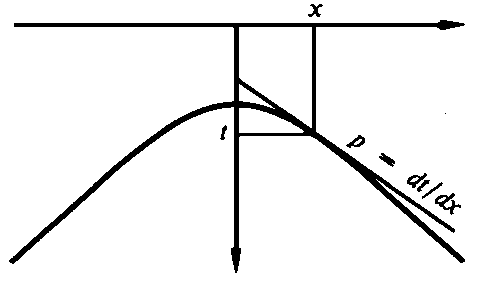
\includegraphics[width=0.65\textwidth]{slnt/tangent}
\caption[tangent]{直线与双曲线时距曲线相切,该直线之斜率p为
任意,因而可取其切点位于信噪比良好之处(据Gonzalez)
}
\label{fig:slnt/tangent}
\end{figure}


要想说明分层介质中的速度,最佳途径就是将它描
述为某种函数$v'(z)$。另一种途径则是挑出某个Snell参
量p并沿具有这个p值的射线开始向下进入地层,当射线
在时刻$t=0$时从地面进入地下时,射线将以速度$v(p,t)$向下移动着。根据$v'(z)$计算
出$v(p,t)$或者由$v(p,t)$计算出$v'(z)$,这属于一种基本性的运算功夫。射线在时间t内旅
行经过的距离x由速度水平分量的时间积分给出,即。
\begin{equation}
x=\int_0^t v(p,t)\sin\theta dt
\label{eq:ex5.4.4}
\end{equation}
以pv代替$\sin\theta$并将常数p提出在积分号外,得
\begin{equation}
x=p\int_0^t[v(p,t)]^2dt
\label{eq:ex5.4.5}
\end{equation}
记住$p=dt/dx$,将\ref{eq:ex5.4.5}代入\ref{eq:ex5.4.3}
\begin{equation}
v_{观测}^2=\frac{x}{t}\frac{dx}{dt}
\label{eq:ex5.4.6}
\end{equation}
则得
\begin{equation}
v_{观测}^2=\frac{1}{t}\int_0^t[v(p,t)]^2dt
\label{eq:ex5.4.7}
\end{equation}
此式证实了下述论断
\begin{equation}
v_{观测}=v_{RMS}
\label{eq:ex5.4.8}
\end{equation}
方程\ref{eq:ex5.4.7}是严格的定义,它无需乎涉及“小炮检距”假设或者“直线射线”假设。

其次让我们来计算层速度。图\ref{fig:slnt/tan2}表示由两个平界面形成的双曲面波至,作两条具有
相同斜率p的直线分别与各该双曲线相切,测定出切点分别为$(x_1,t_1)$和$(x_2,t_2)$。将式
\ref{eq:ex5.4.6}与\ref{eq:ex5.4.4}结合起来,并用下标i表示第i个切点$(x_i,t_i)$,得出
\begin{equation}
x_i\frac{dx}{dt}=\int_0^{t_i}[v(p,t)]^2dt
\label{eq:ex5.4.9}
\end{equation}
假设相继两个同相轴之间的速度为常数$v_{\text{层}}$,于是从具有下标$i+1$
的式\ref{eq:ex5.4.9}中减去具有下标i的式\ref{eq:ex5.4.9},得到
\begin{equation}
(x_{i+1}-x_i)\frac{dx}{dt}=\int_{t_i}^{t_{i+1}}[v(p,t)]^2dt=
(t_{i+1}-t_i)v_{\text{层}}^2
\label{eq:ex5.4.10}
\end{equation}
由此解出层速度$v_{\text{层}}$得
\begin{equation}
v_{\text{层}}^2=\frac{x_{i+1}-x_i}{t_{i+1}-t_i}\frac{dx}{dt}
\label{eq:ex5.4.11}
\end{equation}



\begin{figure}[H]
\centering
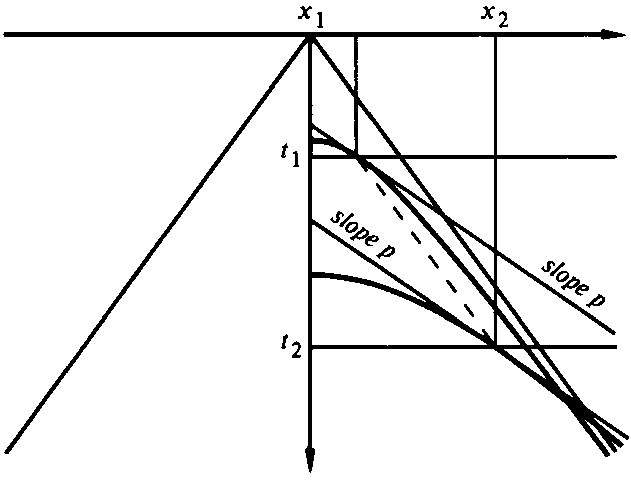
\includegraphics[width=0.65\textwidth]{slnt/tan2}
\caption[tan2]{在共中心点道集上作两条平行直线,使与两个平反射面
形成的反射时距曲线相切(据Gonzalez)
}
\label{fig:slnt/tan2}
\end{figure}

所以,由式\ref{eq:ex5.4.11}可知,利用图\ref{fig:slnt/tan2}中实线直线与虚线直线这两条线的斜率之乘积的
平方根,就可以直接测定出第i反射面与第
$i+1$反射面之间物质的速度。用人工方法在数
据资料上作出两条直线求解层速度的方法优越
于自动速度分析之处在于,你能以图解方式目
估出观测结果对噪音的灵敏度,因而你能在数
据资料中选出最佳炮检距在其上进行观测。

如果你经常性地作这工作,你很快就会发
觉主要工作是要精确作出与各该同相轴相切的
两条直线。当你碰到困难时,你会发现,采用
线性时差校正$t'=t-px$来重新显示数据是有
方便之处的,进行重新显示之后,各直线就不
再是倾斜的而是水平的,这就使得可以使用许
多计时直线中的任何一条直线,现在切点定位
问题变成了一个寻求凸同相轴顶点的问题,这种情形如图\ref{fig:slnt/tan3}所示。

\begin{figure}[H]
\centering
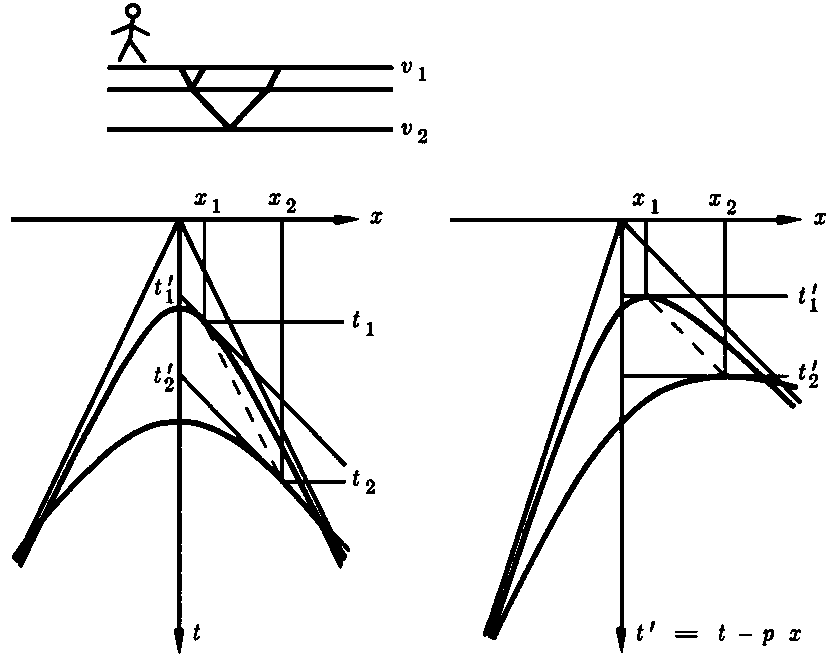
\includegraphics[width=0.65\textwidth]{slnt/tan3}
\caption[tan3]{利用线性时差校正测定层速度(据Gonzalez)
}
\label{fig:slnt/tan3}
\end{figure}

以时间$t'$来表示式\ref{eq:ex5.4.11}则
\begin{equation}
v_{层}^2=\frac{1}{\frac{\Delta t}{\Delta x}}\frac{1}{p}
=\frac{1}{\frac{\Delta t'}{\Delta x}+p}\frac{1}{p}
\label{eq:ex5.4.12}
\end{equation}
在图\ref{fig:slnt/tan3}的右图中测定地层速度,先是测定图中虚线的斜率
即$\Delta t'/\Delta x$,然后把它代入式
\ref{eq:ex5.4.12}内即可。根据用于作图的线性时差校正量大小,已经知道式中的p值。

\subsection{共中心点Snell坐标}
\label{sec:5.4.2}

共中心点倾斜波场分析是一 种比Snell波处理方法更为稳健
的处理地震数据分析的方法,
中心点分析的好处是地层倾角的影响趋向于主要表现在中心点坐标轴上,而地震速度的影响
则主要表现在炮检距坐标轴上。

共中心点分析的缺点在于非物理上可实现。共检波点道集的倾斜叠加模拟的是下行Snell
波,因而你有希望能够写出一个描述该波的微分方程,不管它是多次反射还是横向速度变化,
产生什么结果都没关系。共中心点倾斜叠加则并不模拟物理可实现的任何东西,更不必说存
在有可将这样一种叠加结果进行外推的偏微分方程了,这并不意味着共中心点坐标系统一定
出了什么毛病,但是这点确实使我们更关心Snell波方法了,尽管它在工业界内的应用完全
不是突飞猛进地増长。

值得密切注意的是某些人进行共中心点倾斜叠加比共检波点倾斜叠加还容易,这是因为
在共中心点上,双曲面顶点必然是位于零炮检距上,Fresnel带的位置可以很容易预测出来,
因而内插和丢失数据问题就大大得到缓和。

地震数据是在时间、检波点、炮点和深度坐标系统$(t,g,s,z)$内采集的。现在要定
义一种新的四分量系统,中心点按通常的方式定义
\begin{equation}
y(t,g,s,z)=\frac{g+s}{2}
\label{eq:5.4.13}
\end{equation}
旅行时间深度利用钻井内的垂直相速度$v/\cos\theta$来定义,为尽可能地方便,采用双程旅行时
间$\tau$\footnote{
$\theta$是射线与垂直坐标轴z之间所夹角度。---译者
}。
\begin{equation}
\tau(t,g,s,z)=2z\frac{\cos\theta}{v}
\label{eq:5.4.14}
\end{equation} 
其次定义地面炮检距$h'$,我们将不采用炮检距的老定义。在这种新定义方法情形下,炮点与
检波器不是直接向下移而是沿射线向下移,如$h'$是按下列关系定义的,就可以如此
\begin{equation}
h'(t,g,s,z)=\frac{g-s}{2}+z\tau\theta
\label{eq:ex5.4.15}
\end{equation}
由$h'$的这种新定义可知,在$h'$为常数的情形下,炮点与检波点之间距$(g-s)$将随深度z之
増大而减小。

从点震源观测排列之旅行时间$t$减去相应的线性时差,现将它定义为线性时差校正时间、
或简写为LMO时间(linear moveout
time),因此,在任何深度z时的$LMO$时间等于$t-p
(g-s)$。由于已将h'定义为地表半炮检距,故将t'义为地表LMO时间。根据已延拓至深
度z之排列的LMO时间,再加上该排列的旅行时间深度$\tau$,可把地面上的LMO时间$t'$定义为
\begin{equation}
t'=t-p(g-s)+\tau
\label{eq:5.4.16}
\end{equation}
你也许喜欢将式\ref{eq:5.4.16}
想像成是“斜着”的上行波时间延迟,比如把它看成$t'=t_{lMO}+(z_{slant}/v)$,
不论那种情形,形式上都是
\begin{equation}
t'(t,g,s,z)=t-p(g-s)+2z\frac{\cos\theta}{v}
\label{eq:5.4.17}
\end{equation}
图\ref{fig:slnt/cmplmo}就是这些概念的几何表示。

\begin{figure}[H]
\centering
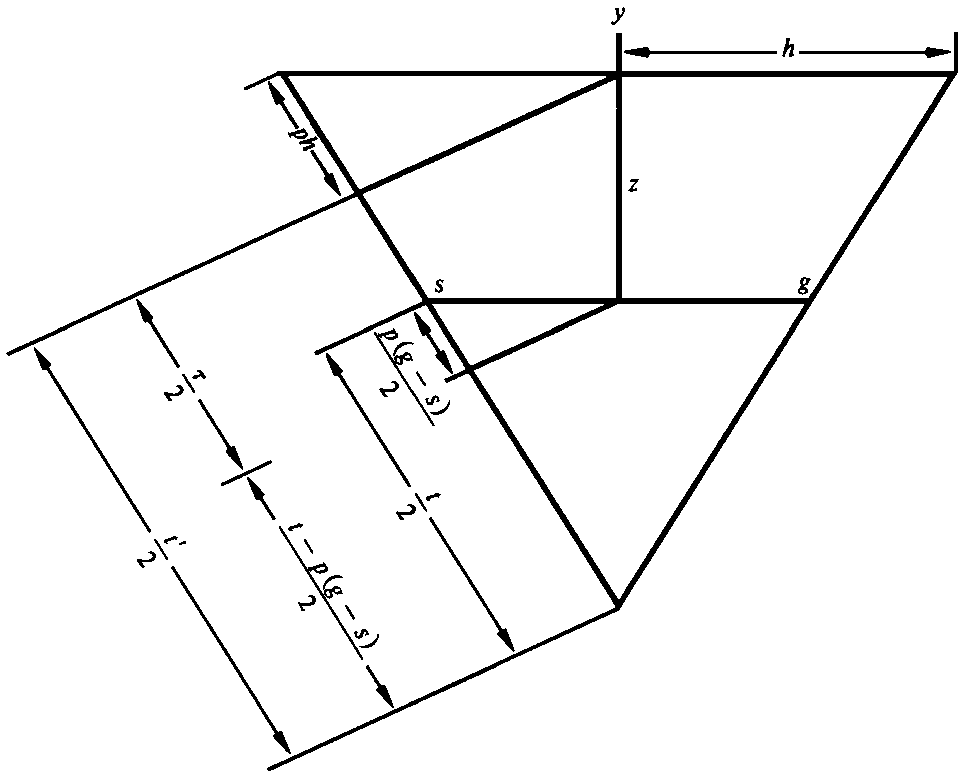
\includegraphics[width=0.65\textwidth]{slnt/cmplmo}
\caption[cmplmo]{共中心点道集与LMO时间坐标框架几何形态,对于描迷类似于一种参考Snell
的各种波场,这是一种很自然的坐标系统
}
\label{fig:slnt/cmplmo}
\end{figure}

由图\ref{fig:slnt/cmplmo}所示几何关系将得出结论:观测某个特定值$(h',t')$时的反射,直接就可确定
速度。反射面深度之方程可写出为
\begin{equation}
\text{反射面深度}=\frac{h'}{\tan\theta}=v(\frac{t'}{2}+ph')\cos\theta
\label{eq:ex5.4.18}
\end{equation}

利用Snell定律消去其中的角度,然后解出速度,得
\begin{equation}
v^2=\frac{1}{p}\frac{1}{p+\frac{t'}{2h'}}
\label{eq:ex5.4.19}
\end{equation}
此式同式\ref{eq:ex5.4.12}完全一致。

将上述各项定义集中为一组方程,并以遍及z的积分来代替z以便允许速度随
深度而变化,我们得出:
\begin{subequations}
\begin{equation}
t'(t,g,s,z)=t-(g-s)+2\int_0^z\frac{\cos\theta}{v}dz
\label{eq:ex5.4.20a}
\end{equation}
\begin{equation}
y(t,g,s,z)=\frac{g+s}{2}
\label{eq:ex5.4.20b}
\end{equation}
\begin{equation}
h'(t,g,s,z)=\frac{g-s}{2}+\int_0^z\tan\theta dz
\label{eq:ex5.4.20c}
\end{equation}
\begin{equation}
\tau(t,g,s,z)=2\int_0^z\frac{\cos\theta}{v}dz
\label{eq:ex5.4.20d}
\end{equation}
\label{eq:ex5.4.20}
\end{subequations}


在使用这些方程以前,必须按照层状介质情形下的Snell定律$\sin\theta(z)=pv(z)$把所有三
角函数从式中消去,Snell参量p在整个分析过程中均为一常数值。

把由\ref{eq:ex5.4.20a}得出的$dt'/dz$和由\ref{eq:ex5.4.20c}得出的
$dh'/dz$结合起来时,得
\begin{equation}
\frac{dt'}{dh'}=\frac{2\cos\theta}{v\tan\theta}
\label{eq:ex5.4.21}
\end{equation}
根据关系式$pv=\sin\theta$消去式中的三角函数,就可使我们解出层速度为
\begin{equation}
v^2=\frac{1}{p}\frac{1}{p+\frac{1}{2}\frac{dt'}{dh'}}
\label{eq:ex5.4.22}
\end{equation}
这又一次得出了测定层速度的方程\ref{eq:ex5.4.12}。

位于地表面$z=0$时,仅需对p作出数值选择然后进行线性时差校正,即可将地震勘探资
料以坐标框架\ref{eq:ex5.2.20}表示。迄今尚无须要求有关速度$v(z)$的知识。接着我们来查找某
些歪斜双曲线顶部的数据,找出一些后,我们就利用方程\ref{eq:ex5.4.12}、\ref{eq:ex5.4.19}或者\ref{eq:ex5.4.22} 求出某种速度,采用这种速度开始作向下延拓处理。

波场可以在物理坐标系统$(t,g,s,z)$或新定义的坐标系统$(t',y,h',\tau)$内描述,在
物理坐标系统内,成像在
\begin{equation}
t=0 \quad \text{及}\quad g=s
\label{eq:ex5.4.23}
\end{equation}
时出现。为在Snell坐标内表达这些条件,将式\ref{eq:ex5.4.23}代进\ref{eq:ex5.4.20a}与
\ref{eq:ex5.4.20d}
内,所得结果就是程序人员所谓的停机条件
\begin{equation}
t'=\tau
\label{eq:ex5.4.24}
\end{equation}
这是速度信息应当被最佳聚焦于$(h',t')$平面时的深度。下面我们将讨论某些向下延拓方程。

\subsection{微分方程与Fourier变换}
\label{sec:5.4.3}

由偏微分方程的连锁法得出
\begin{equation}
\begin{pmatrix}
\partial_t\\
\partial_g\\
\partial_s\\
\partial_z
\end{pmatrix}=
\begin{pmatrix}
t_t' & y_t & h_t' & \tau_t \\
t_g' & y_g & h_g' & \tau_g \\
t_s' & y_s & h_s' & \tau_s \\
t_z' & y_z & h_z' & \tau_z
\end{pmatrix}
\begin{pmatrix}
\partial_t'\\
\partial_y\\
\partial_h\\
\partial_\tau
\end{pmatrix}
\label{eq:ex5.4.25}
\end{equation}
按我们通常的符号,时间导数$\partial_t$的Fourier表象是$-i\omega$,与此类似,$\partial_t'$及空间导数$
\partial_h',\partial_\tau,\partial_g,\partial_g,\partial_z)$
的相应表象分别为$-i\omega '$及$i(k_y,k_h',k_\tau,k_g,k_s,k_z)$。在矩阵关系\ref{eq:ex5.4.25}
的两个列向量中采用这些Fourier变量并对方程\ref{eq:ex5.4.20}微分,求出矩阵\ref{eq:ex5.4.25}中的 各元素,得到下述矩阵关系
\begin{equation}
\begin{pmatrix}
-\omega\\
\k_g\\
\k_s\\
\k_z
\end{pmatrix}=
\begin{pmatrix}
1 & 0 & 0 & 0 \\
-p & \frac{1}{2} & \frac{1}{2} & 0 \\
p & \frac{1}{2} & -\frac{1}{2} & 0 \\
\frac{2\cos\theta}{v} & 0 & \tan\theta & \frac{2\cos\theta}{v}
\end{pmatrix}
\begin{pmatrix}
-\omega '\\
k_y\\
k_h'\\
k_\tau
\end{pmatrix}
\label{eq:ex5.4.26}
\end{equation}
设S为震源处的入射角之正弦,G为检波点处的出射角之正弦。如速度v已知,则由共检
波点道集和共炮点道集上的时差可分别直接测定出这些角度。与此类似,在共炮检距剖面上
或倾斜叠加剖面上所观测到的时差应与视倾角Y有关,在经过线性时差校正的共中心点道集
上由时差所测量出的是视时差H'。其精确定义分别为
\begin{subequations}
\begin{equation}
S=\frac{vk_s}{\omega}, G=\frac{vk_g}{\omega}
\label{eq:ex5.4.27a}
\end{equation}
\begin{equation}
Y=\frac{vk_y}{2\omega}, H'=\frac{vk_h'}{2\omega}
\label{eq:ex5.4.27b}
\end{equation}
\label{eq:ex5.4.27}
\end{subequations}
利用矩阵\ref{eq:ex5.4.26}中的相应一些定义可得出下述关系
\begin{subequations}
\begin{equation}
G=pv+Y+H'=Y+(H'+pv)
\label{eq:ex5.4.28a}
\end{equation}
\begin{equation}
S=-pv+Y-H'=Y-(H'+pv)
\label{eq:ex5.4.28b}
\end{equation}
\label{eq:ex5.4.28}
\end{subequations}
利角关系式$H'=H-pv$就可将人们熟悉的炮检距时差角H同LMO剩余时差角H'联系起来。
令H'等于零意味着是令$k_h'$等于零,从而暗示遍及$h'$进行了积分,这最终也就是暗示以倾斜
角p对数据进行倾斜叠加。$H'/v$值或$k_h'/\omega$值很小就是指时差接近于p。


\subsection{处理的可能性}
\label{sec:5.4.4}

双平方根方程(DSR)为
\begin{equation}
\frac{k_x}{\omega}=-\frac{1}{v}(\sqrt{1-S^2}+\sqrt{1-G^2})
\label{eq:ex5.4.29}
\end{equation}
代入\ref{eq:ex5.4.26}及\ref{eq:ex5.4.27a},该双平方根方程变为
\begin{equation}
\frac{k_\tau}{\omega}=1-\frac{pv}{1-p^2v^2}H'-\frac{1}{2}\{
[1-\frac{2pv(H'-Y)+(H'-Y)^2}{1-p^2v^2}]^\frac{1}{2}+
[1-\frac{2pv(H'+Y)+(H'+Y)^2}{1-p^2v^2}]^\frac{1}{2}\}
\label{eq:ex5.4.30}
\end{equation}

方程\ref{eq:ex5.4.30}就是以所谓延迟Snell中心点坐标形式表示的双平方根方程
之准确表达式。

坐标系统\ref{eq:ex5.4.20}可以描述任何介质内的任何波场,不过,在射线大体平行于具有所
选Snell参量p的任何射线的情形下,只有在速度接近于$v(z)$的层状介质内,方程\ref{eq:ex5.4.20}
才有特别好处。除非坐标系统“配得上”正在研究的波,不然没多少理由婆采用这些坐榇,
所谓配得上的波就是参量接近于所选p值的那些波,这意味着不可过大。对式\ref{eq:ex5.4.30}
有可能作种种简化展开,在三种构成因素和r中间的量值不等关系有许多种不同排
列方法,你要按照具体条侔选取展开方法。然而关
于如何展开才适当以及生产上应作何考虑
等问题迄今尚说不出一个完整的轮廓梗概,不过,让我们考虑一下两种可能性。

首先,任何数据集可以按时差分解成许多数据集,每种数据集在时差空间一例如在共
中心点道集倾斜叠加中---内都具有狹频带,对这些数据集中的任何一个来说,都完全
可忽略不计,这时方程\ref{eq:ex5.4.30}将筒化为
\begin{subequations}
\begin{equation}
\frac{k_\tau}{\omega}=1-\frac{1}{2}\{
[1-\frac{-2pvY + Y^2}{1-p^2v^2}]^\frac{1}{2}+
[1-\frac{+2pvY + Y^2}{1-p^2v^2}]^\frac{1}{2}\}
\label{eq:ex5.4.31a}
\end{equation}
或者
\begin{equation}
\frac{k_\tau}{\omega}=1-\frac{1}{2\sqrt{1-p^2v^2}}
[\sqrt{1-(Y-pv)^2}+\sqrt{1-(Y+pv)^2}]
\label{eq:ex5.4.31b}
\end{equation}
\label{eq:ex5.4.31}
\end{subequations}
上述处理方法类似于Richard Ottolini在其学位论文中所使用过的一种方法。

其次,让我们给式\ref{eq:ex5.4.30}补充一种近似关系,使其中的Y与H'可单独分离出来。我们
将采用\ref{sec:3.4}节介绍过的分离法。式\ref{eq:ex5.4.30}是这个近似关系的第一部分,这时取$Y=0$并保
持$H'$的直至二次项之所有的项,得
\begin{equation}
\frac{k_\tau}{\omega}=\frac{H'^2}{2(1-p^2v^2)^2}
\label{eq:ex5.4.32}
\end{equation}

式\ref{eq:ex5.4.30}的分离近似就是式\ref{eq:ex5.4.31b}加上式\ref{eq:ex5.4.32}。式\ref{eq:ex5.4.32}中不存
在的线性项并不令人感到意外,坐标系统已经设计成使得在所选模型$Y=0$与$H=pv$附近
的能量在向下延拓进行的时候不应当在$(h',t')$平面内有漂移。

方程\ref{eq:ex5.4.32}所代表的速度谱概念就是利用H'项使数据在$(h',t')$平面上聚焦,在
聚焦之后,应有可能按照使道集上的同相轴衔接起来的斜率而直接读出层速度。这种办法在
Alfonso Gonzalez(1982)的学位论文中曾经使用过。

\subsection{习题}
\label{sec:5.4.5}


 \begin{enumerate}
\item 设零炮检距剖面上已识别岀某个双曲线,顶部模糊不清,但你尚可在两个位置上
测定$(p,x,t)$,试求地层速度。已知在野外剖面上有相同测定结果(s为恒定),试求地层
速度。

\end{enumerate}













